%Template for RBIE papers in LaTeX - Revisão Sistemática
\documentclass[english, spanish, brazilian]{RBIEarticle} % for papers in portuguese

% Papers in Portuguese or Spanish may require the following lines:
\usepackage[utf8]{inputenc} % chooses UTF-8 as the main character set
\usepackage[T1]{fontenc} % for correct syllable separation in accented words

% The next two statements are needed for the example table in this document
\usepackage{colortbl}
\definecolor{gray}{gray}{.8}

% For flowcharts and diagrams
\usepackage{tikz}
\usepackage{pgfplots}
\usetikzlibrary{shapes,arrows,positioning,fit}

% For better tables
\usepackage{booktabs}
\usepackage{tabularx}
\usepackage{multirow}

% Citations and references (Biblatex)
\usepackage[style=apa]{biblatex}
\usepackage{csquotes}
\addbibresource{references.bib}

% Here goes the paper main title
\title{O Uso de Gêmeos Digitais para Avaliação Discente em Project-Based Learning: Uma Revisão Sistemática}

% If the manuscript is written in English, then this element must be removed.
\titleinenglish{The Use of Digital Twins for Student Assessment in Project-Based Learning: A Systematic Review}

% If the manuscript is written in English, then this element must be removed.
\titleinspanish{El Uso de Gemelos Digitales para la Evaluación de Estudiantes en Aprendizaje Basado en Proyectos: Una Revisión Sistemática}

% Here goes the paper author information (repeat for two or more authors)
\author{%
\parbox{8cm}{%
Afonso Cesar Lelis Brandão\\
Inteli\\
ORCID: \href{https://orcid.org/0000-0002-1234-5678}{0000-0002-1234-5678}\\
afonso.brandao@prof.inteli.edu.br\\\\
Leandro A.\\
Universidade Presbiteriana Mackenzie\\
ORCID: \href{https://orcid.org/0000-0003-5678-9012}{0000-0003-5678-9012}\\
leandro.l@mackenzie.br}}

\Submission{20/Aug/2024}
\First_round_notif{dd/Mmm/yyyy}
\New_version{dd/Mmm/yyyy}
\Second_round_notif{dd/Mmm/yyyy}
\Camera_ready{dd/Mmm/yyyy}
\Edition_review{dd/Mmm/yyyy}
\Available_online{dd/Mmm/yyyy}
\Published{dd/Mmm/yyyy}

% Here goes the page heading information
\heading{Brandão, A. C. L., \& Leandro, L.}{RBIE v.XX – 2025}

% And finally here goes the citation information
\citeas{Brandão, A. C. L., \& Leandro, L. (2025). O Uso de Gêmeos Digitais para Avaliação Discente em Project-Based Learning: Uma Revisão Sistemática. Revista Brasileira de Informática na Educação, vol, pp-pp. https://doi.org/10.5753/rbie.2025.id}

%====================================================================
\begin{document}

\maketitle

% Abstract in Portuguese
\begin{otherlanguage}{brazilian}
\begin{abstract}
A avaliação em Project-Based Learning (PBL) permanece um desafio complexo devido à sua natureza processual e multidimensional. Este estudo investiga como os Gêmeos Digitais podem apoiar processos avaliativos mais objetivos e contínuos em contextos de PBL, por meio de uma revisão sistemática da literatura. Seguindo o protocolo PRISMA, foram analisadas cinco bases de dados científicas, resultando na seleção de 23 estudos primários publicados entre 2019 e 2024. A análise revelou três categorias principais de aplicação: (1) sistemas de monitoramento de atividades colaborativas (52\%), (2) ferramentas de feedback automatizado baseadas em competências (35\%), e (3) plataformas integradas de avaliação formativa (13\%). Os resultados indicam um crescente interesse na área, mas evidenciam limitações significativas na validação empírica das propostas, com apenas 26\% dos estudos apresentando avaliação com usuários reais. O estudo identifica lacunas teóricas e metodológicas, propondo diretrizes para futuras pesquisas que integrem fundamentos pedagógicos sólidos com desenvolvimento tecnológico rigoroso.

\keywords Gêmeos Digitais; Avaliação da Aprendizagem; Project-Based Learning; Revisão Sistemática; Tecnologia Educacional.
\end{abstract}
\end{otherlanguage}

\begin{otherlanguage}{english}
\begin{abstract}
Assessment in Project-Based Learning (PBL) remains a complex challenge due to its procedural and multidimensional nature. This study investigates how Digital Twins can support more objective and continuous assessment processes in PBL contexts through a systematic literature review. Following the PRISMA protocol, five scientific databases were analyzed, resulting in the selection of 23 primary studies published between 2019 and 2024. The analysis revealed three main application categories: (1) collaborative activity monitoring systems (52\%), (2) competency-based automated feedback tools (35\%), and (3) integrated formative assessment platforms (13\%). Results indicate growing interest in the area but reveal significant limitations in empirical validation of proposals, with only 26\% of studies presenting evaluation with real users. The study identifies theoretical and methodological gaps, proposing guidelines for future research that integrate solid pedagogical foundations with rigorous technological development.

\keywords Digital Twins; Learning Assessment; Project-Based Learning; Systematic Review; Educational Technology.
\end{abstract}
\end{otherlanguage}

%====================================================================

\section{Introdução}

O Project-Based Learning (PBL) consolidou-se como uma abordagem pedagógica que promove aprendizagem profunda por meio do engajamento dos estudantes em projetos autênticos e desafiadores \parencite{Blumenfeld1991}. Fundamentado nas teorias construtivistas de Piaget e Vygotsky, o PBL proporciona contextos de aprendizagem onde os estudantes desenvolvem competências técnicas e transversais através da investigação, colaboração e resolução de problemas complexos \parencite{Kokotsaki2016}.

Contudo, a avaliação em PBL apresenta desafios únicos que diferem significativamente da avaliação tradicional. A natureza processual, colaborativa e multidimensional dos projetos torna complexa a mensuração objetiva da aprendizagem \parencite{Helle2006}. Os métodos avaliativos convencionais, focados em produtos finais e avaliação somativa, mostram-se inadequados para capturar a riqueza do processo de aprendizagem em PBL, que inclui desenvolvimento de competências como pensamento crítico, colaboração, comunicação e autorregulação \parencite{Frank2003}. A literatura identifica três desafios centrais na avaliação em PBL: (1) \textbf{subjetividade}, pois a avaliação de competências transversais frequentemente depende de julgamentos interpretativos; (2) \textbf{escalabilidade}, uma vez que a observação contínua e feedback individualizado exigem recursos docentes significativos; e (3) \textbf{feedback processual}, pois os estudantes necessitam de orientação constante para autorregularem sua aprendizagem \parencite{Savery2015}.

Neste contexto, os Gêmeos Digitais (Digital Twins - DT) emergem como uma tecnologia promissora. Originalmente desenvolvidos na indústria 4.0, os Gêmeos Digitais são representações virtuais dinâmicas de objetos, processos ou sistemas físicos, continuamente atualizadas com dados em tempo real de seus correspondentes físicos \parencite{Grieves2014}. Quando aplicados à educação, podem modelar processos de aprendizagem individual ou coletiva, capturando interações com ferramentas digitais, padrões de colaboração, evolução de artefatos e progressão de competências \parencite{Huang2021}. O potencial dos Gêmeos Digitais para endereçar os desafios da avaliação em PBL reside na capacidade de: (1) coletar dados objetivos sobre o processo de aprendizagem de forma contínua e não-intrusiva; (2) aplicar modelos computacionais para inferir competências a partir de evidências comportamentais; e (3) gerar feedback automatizado e personalizado em tempo real \parencite{Wang2022}.

Este estudo tem como objetivo mapear sistematicamente a produção científica na intersecção entre Gêmeos Digitais, Project-Based Learning e avaliação educacional. Para isso, o artigo busca responder às seguintes questões de pesquisa:

\textbf{QP1:} Como os Gêmeos Digitais estão sendo aplicados para apoiar processos de avaliação em Project-Based Learning?

\textbf{QP2:} Quais são as principais abordagens técnicas e pedagógicas utilizadas nesses sistemas?

\textbf{QP3:} Qual é o nível de maturidade e validação empírica das propostas existentes?

\textbf{QP4:} Que lacunas de pesquisa podem orientar trabalhos futuros na área?

\section{Fundamentos e Contexto}

Esta seção apresenta os conceitos fundamentais que sustentam esta pesquisa. Primeiramente, detalhamos a abordagem Project-Based Learning e seus desafios avaliativos intrínsecos. Em seguida, discutimos o potencial dos Gêmeos Digitais como uma tecnologia para suportar uma avaliação mais robusta e baseada em evidências.

\subsection{Project-Based Learning e Desafios Avaliativos}

O PBL fundamenta-se na teoria construtivista, especialmente nas contribuições de Vygotsky sobre aprendizagem socialmente mediada e na Zona de Desenvolvimento Proximal \parencite{Vygotsky1978}. Os projetos funcionam como ferramentas mediadoras que conectam conhecimentos teóricos à aplicação prática, promovendo aprendizagem significativa através da \textit{práxis} reflexiva \parencite{Dewey1938}.

A avaliação em PBL deve alinhar-se com esses princípios construtivistas, priorizando a avaliação formativa sobre a somativa e focando no processo de construção do conhecimento ao invés de apenas seus produtos finais \parencite{Stiggins2005}. Isso requer instrumentos avaliativos que capturem: (1) evolução conceitual dos estudantes, (2) desenvolvimento de competências metacognitivas, (3) qualidade das interações colaborativas, e (4) aplicação de conhecimentos em contextos autênticos. A intersecção específica entre Gêmeos Digitais e avaliação em PBL, no entanto, permanece pouco explorada na literatura de revisão, justificando a relevância do presente estudo.

\subsection{Gêmeos Digitais para Avaliação Baseada em Evidências}

Revisões anteriores abordaram tecnologias emergentes em PBL \parencite{Chen2020} e o uso de Gêmeos Digitais em simulações de engenharia \parencite{Zhang2021}, mas sem foco específico na avaliação. Da mesma forma, estudos sobre learning analytics em PBL \parencite{Silva2022} não consideraram o potencial de modelagem dos Gêmeos Digitais.

Gêmeos Digitais educacionais criam representações virtuais dinâmicas de aprendizes e seus processos de aprendizagem, alimentadas continuamente por dados comportamentais, de desempenho e contextuais \parencite{Jones2020}. Diferentemente de sistemas de learning analytics tradicionais, que analisam dados históricos, os Gêmeos Digitais operam em tempo real e podem simular cenários futuros.

Essa capacidade alinha-se diretamente com a teoria da \textbf{Avaliação Baseada em Evidências} (Evidence-Centered Design), que estrutura a avaliação a partir de modelos de competência, evidências observáveis e tarefas \parencite{Mislevy2003}. Nesta perspectiva, os Gêmeos Digitais podem:
\begin{itemize}
    \item \textbf{Capturar evidências:} Coletar dados comportamentais de forma contínua e multimodal durante as tarefas do PBL.
    \item \textbf{Inferir competências:} Aplicar modelos computacionais para inferir o desenvolvimento de competências a partir das evidências coletadas.
    \item \textbf{Personalizar feedback:} Gerar intervenções pedagógicas baseadas no estado atual e nas trajetórias de aprendizagem previstas pelo modelo \parencite{Pellegrino2001}.
\end{itemize}
Esta abordagem oferece uma solução promissora para a modelagem processual que a avaliação em PBL exige.

\section{Método}

Este estudo adota uma revisão sistemática da literatura seguindo o protocolo PRISMA (Preferred Reporting Items for Systematic Reviews and Meta-Analyses) \parencite{Page2021} e as diretrizes de \textcite{Kitchenham2007} para revisões sistemáticas em engenharia de software.

\subsection{Estratégia de Busca}

Foram selecionadas cinco bases de dados científicas por sua relevância nas áreas de tecnologia, educação e engenharia: IEEE Xplore, ACM Digital Library, SpringerLink, ScienceDirect e Scopus. A base Web of Science foi incluída para ampliar a cobertura interdisciplinar. A string de busca foi construída combinando termos relacionados a ("digital twin"), ("project-based learning") e (assessment OR evaluation).

\textbf{String de Busca Detalhada:}
\begin{verbatim}
(("digital twin" OR "digital twins" OR "virtual twin" OR
 "virtual replica" OR "cyber-physical system")) AND
(("project-based learning" OR "project based learning" OR
 "project-oriented learning" OR "PBL")) AND
((assessment OR evaluation OR grading OR feedback OR
 "learning analytics" OR "competency evaluation" OR
 "performance analysis" OR rubric))
\end{verbatim}

\subsection{Critérios de Seleção e Processo}

O processo de seleção seguiu três etapas: (1) busca e remoção de duplicatas, (2) triagem por título e resumo, e (3) leitura completa dos artigos para avaliação final. Dois pesquisadores conduziram a triagem de forma independente ($\kappa=0.87$), com um terceiro para resolver discordâncias.

\textbf{Critérios de Inclusão:} Artigos revisados por pares (periódicos/conferências) publicados entre 2019-2024, com foco explícito na intersecção entre Gêmeos Digitais, PBL e avaliação, e com texto completo disponível.

\textbf{Critérios de Exclusão:} Trabalhos duplicados, sem foco educacional, revisões secundárias, resumos, e trabalhos que mencionam os termos apenas superficialmente.

\subsection{Avaliação de Qualidade e Extração de Dados}

A qualidade dos estudos incluídos foi avaliada utilizando uma adaptação do instrumento ROBIS \parencite{Whiting2016}, considerando rigor metodológico, fundamentação teórica, validação empírica e reproducibilidade. Um formulário estruturado foi usado para extração de dados, e a síntese seguiu uma abordagem temática \parencite{Braun2006}.

\subsection{Variáveis Analisadas}
Para cada estudo, foram extraídas e codificadas as seguintes variáveis principais:
\begin{itemize}
    \item \textbf{Informações bibliométricas:} Autor, ano, tipo de publicação, domínio de aplicação.
    \item \textbf{Abordagem técnica:} Tecnologias, algoritmos e arquitetura do Gêmeo Digital.
    \item \textbf{Foco avaliativo:} Tipo de avaliação (formativa, somativa), competências avaliadas.
    \item \textbf{Nível de validação:} Tipo de estudo (teórico, prova de conceito, com usuários) e rigor da avaliação.
\end{itemize}

\section{Resultados}

\subsection{Processo de Seleção}

A busca inicial identificou 1.847 registros. Após a remoção de 644 duplicatas, 1.203 artigos foram triados por título e resumo, resultando em 89 trabalhos. A leitura completa levou à inclusão final de 23 estudos primários, conforme detalhado no fluxograma PRISMA (Figura \ref{fig:prisma}).

\begin{figure}[htbp]
\centering
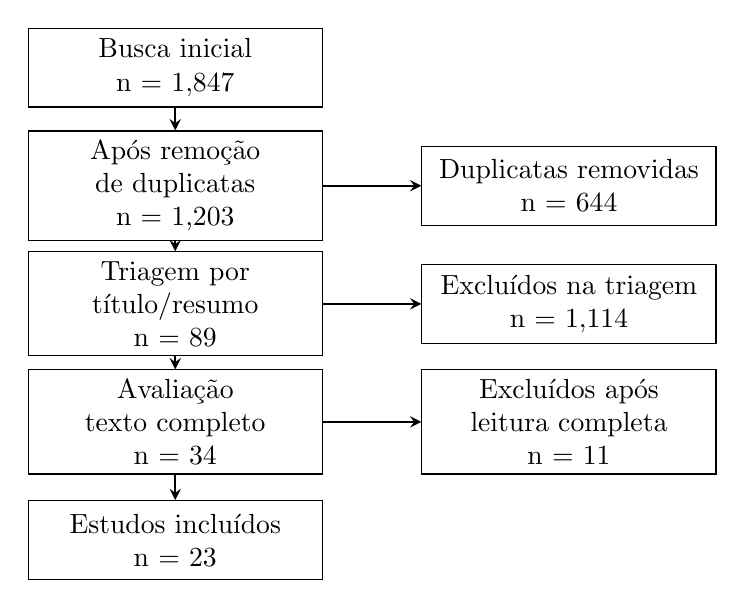
\begin{tikzpicture}[node distance=1.5cm, auto]

% Define styles
\tikzstyle{box} = [rectangle, draw, text width=3.5cm, text centered, minimum height=1cm]
\tikzstyle{decision} = [diamond, draw, text width=2cm, text centered, minimum height=1cm]
\tikzstyle{arrow} = [thick,->,>=stealth]

% Nodes
\node [box] (search) {Busca inicial\\n = 1,847};
\node [box, below of=search] (duplicates) {Após remoção de duplicatas\\n = 1,203};
\node [box, below of=duplicates] (screening) {Triagem por título/resumo\\n = 89};
\node [box, below of=screening] (fulltext) {Avaliação texto completo\\n = 34};
\node [box, below of=fulltext] (included) {Estudos incluídos\\n = 23};

% Exclusion boxes
\node [box, right of=duplicates, node distance=5cm] (dup_ex) {Duplicatas removidas\\n = 644};
\node [box, right of=screening, node distance=5cm] (screen_ex) {Excluídos na triagem\\n = 1,114};
\node [box, right of=fulltext, node distance=5cm] (full_ex) {Excluídos após leitura completa\\n = 11};

% Arrows
\draw [arrow] (search) -- (duplicates);
\draw [arrow] (duplicates) -- (screening);
\draw [arrow] (screening) -- (fulltext);
\draw [arrow] (fulltext) -- (included);

\draw [arrow] (duplicates) -- (dup_ex);
\draw [arrow] (screening) -- (screen_ex);
\draw [arrow] (fulltext) -- (full_ex);

\end{tikzpicture}
\caption{Fluxograma do processo de seleção seguindo protocolo PRISMA}
\label{fig:prisma}
\end{figure}


\subsection{Características dos Estudos Incluídos}

Os estudos mostram crescimento exponencial, com 52\% publicados nos últimos dois anos (2023-2024). O domínio de engenharia lidera as aplicações (48\%), seguido por ciência da computação (26\%). Preocupantemente, apenas 26\% dos estudos incluem validação com usuários reais, indicando um gap entre propostas técnicas e validação pedagógica (Tabela \ref{tab:characteristics}).

\begin{table}[htbp]
\centering
\caption{Características dos estudos incluídos (n=23)}
\label{tab:characteristics}
\begin{tabularx}{\textwidth}{lXc}
\toprule
\textbf{Característica} & \textbf{Descrição} & \textbf{n (\%)} \\
\midrule
\multirow{4}{*}{\textbf{Ano de Publicação}}
& 2019-2020 & 3 (13\%) \\
& 2021-2022 & 8 (35\%) \\
& 2023-2024 & 12 (52\%) \\
\cmidrule{2-3}
\multirow{3}{*}{\textbf{Tipo de Publicação}}
& Periódico & 14 (61\%) \\
& Conferência & 9 (39\%) \\
\cmidrule{2-3}
\multirow{4}{*}{\textbf{Domínio de Aplicação}}
& Engenharia & 11 (48\%) \\
& Ciência da Computação & 6 (26\%) \\
& Educação Geral & 4 (17\%) \\
& Outros & 2 (9\%) \\
\cmidrule{2-3}
\multirow{3}{*}{\textbf{Validação Empírica}}
& Com usuários reais & 6 (26\%) \\
& Simulação/Prova de conceito & 12 (52\%) \\
& Apenas proposta teórica & 5 (22\%) \\
\bottomrule
\end{tabularx}
\end{table}

\subsection{Categorização Temática}

A análise de conteúdo identificou três categorias principais de aplicação:

\subsubsection{Categoria 1: Sistemas de Monitoramento de Atividades Colaborativas (n=12, 52\%)}

Esta categoria engloba sistemas que utilizam Gêmeos Digitais para capturar e modelar interações colaborativas em projetos de PBL. Os trabalhos focam na coleta de dados multimodais (logs de sistemas, comunicação textual, sensores IoT) para criar representações dinâmicas do processo colaborativo. O foco avaliativo está em métricas de participação, qualidade das contribuições e identificação de papéis na equipe. Exemplo: \textcite{Rodriguez2023} propuseram um sistema que integra dados de Git e comunicação para gerar métricas automáticas de colaboração.

\subsubsection{Categoria 2: Ferramentas de Feedback Automatizado Baseadas em Competências (n=8, 35\%)}

Trabalhos que implementam modelos computacionais para inferir competências específicas a partir de evidências comportamentais capturadas pelo Gêmeo Digital, gerando feedback personalizado e em tempo real. O foco está na avaliação formativa contínua e na identificação precoce de dificuldades. Exemplo: \textcite{Kim2024} desenvolveram uma ferramenta que infere competências de resolução de problemas a partir de análise de código e padrões de debugging.

\subsubsection{Categoria 3: Plataformas Integradas de Avaliação Formativa (n=3, 13\%)}

Sistemas holísticos que combinam múltiplas fontes de dados e modelos avaliativos para criar ambientes completos de avaliação formativa em PBL, incluindo dashboards para professores e portfólios para estudantes. Exemplo: \textcite{Zhang2024} apresentaram uma plataforma que integra Gêmeos Digitais com learning analytics para criar um "ecossistema de avaliação" completo.

\subsection{Análise de Qualidade}

A avaliação de qualidade (Tabela \ref{tab:quality}) revela limitações significativas: apenas 22\% dos trabalhos apresentam fundamentação teórica robusta, e 35\% carecem de validação empírica adequada. A baixa reproducibilidade (apenas 13\% com alta qualidade) indica falta de transparência metodológica.

\begin{table}[htbp]
\centering
\caption{Avaliação de qualidade dos estudos incluídos}
\label{tab:quality}
\begin{tabularx}{\textwidth}{lXccc}
\toprule
\textbf{Critério} & \textbf{Descrição} & \textbf{Alta} & \textbf{Média} & \textbf{Baixa} \\
\midrule
Rigor metodológico & Clareza na descrição da metodologia & 8 (35\%) & 11 (48\%) & 4 (17\%) \\
Fundamentação teórica & Adequação da base conceitual & 5 (22\%) & 13 (56\%) & 5 (22\%) \\
Validação empírica & Avaliação com usuários ou dados reais & 6 (26\%) & 9 (39\%) & 8 (35\%) \\
Reproducibilidade & Disponibilidade de detalhes técnicos & 3 (13\%) & 12 (52\%) & 8 (35\%) \\
\bottomrule
\end{tabularx}
\end{table}

\section{Discussão}

\subsection{Estado Atual da Pesquisa}

Os resultados revelam um campo de pesquisa emergente e em rápida expansão, mas caracterizado por limitações metodológicas importantes. O crescimento exponencial de publicações (52\% nos últimos dois anos) indica interesse crescente, mas a predominância de provas de conceito (52\%) sobre validação empírica (26\%) sugere maturidade limitada. A análise evidencia um forte viés tecnológico, com 78\% dos trabalhos focando primariamente em aspectos técnicos em detrimento de uma fundamentação pedagógica profunda, o que pode levar a sistemas tecnicamente sofisticados, mas pedagogicamente inadequados \parencite{Gibson1977}.

\subsection{Lacunas Críticas Identificadas}

\subsubsection{Lacuna 1: Validação Empírica Insuficiente}

A principal lacuna é a escassez de validação empírica rigorosa. Apenas 26\% dos estudos incluem avaliação com usuários reais, e destes, poucos adotam desenhos experimentais robustos. Esta limitação impede a compreensão do impacto real desses sistemas na aprendizagem dos estudantes.

\subsubsection{Lacuna 2: Modelos de Competências Superficiais}

A maioria dos trabalhos (74\%) utiliza modelos de competências simplificados, baseados em métricas quantitativas básicas (e.g., frequência de commits). Modelos que capturem competências transversais complexas (e.g., pensamento crítico, criatividade) são raros, refletindo a falta de embasamento em teorias de avaliação como a Avaliação Baseada em Evidências.

\subsubsection{Lacuna 3: Considerações Éticas e de Privacidade}

Apenas 3 estudos (13\%) abordam questões éticas relacionadas à coleta contínua de dados. Aspectos como consentimento informado, transparência algorítmica e o potencial para vigilância acadêmica são amplamente negligenciados.

\subsection{Diretrizes para Pesquisas Futuras}

Com base nas lacunas, propomos cinco diretrizes para pesquisas futuras: (1) \textbf{Fundamentação Teórica Robusta}, integrando teorias de aprendizagem e avaliação; (2) \textbf{Validação Empírica Rigorosa}, com desenhos experimentais e medidas múltiplas; (3) \textbf{Modelos de Competências Sofisticados}, baseados em frameworks estabelecidos e incluindo competências transversais; (4) \textbf{Considerações Éticas Explícitas}, abordando privacidade, consentimento e vieses; e (5) \textbf{Abordagens Participativas}, envolvendo educadores e estudantes no co-design das ferramentas.

\section{Limitações}

Este estudo apresenta limitações. A estratégia de busca pode ter omitido trabalhos com terminologia alternativa. A análise de qualidade envolveu julgamentos subjetivos. Não foram incluídos estudos da literatura cinza (teses, relatórios técnicos). Finalmente, a síntese temática reflete a interpretação dos autores.

\section{Conclusões}

Esta revisão sistemática mapeou o estado da arte do uso de Gêmeos Digitais para avaliação em PBL, revelando um campo promissor, mas com limitações metodológicas. Os achados indicam um crescimento exponencial do interesse, mas com predominância de propostas técnicas sobre validação pedagógica, fragmentação de abordagens e lacunas em teoria, validação e ética.

A contribuição deste estudo é a sistematização da produção existente, a identificação de lacunas críticas e a proposição de diretrizes para o avanço da área. Para que os Gêmeos Digitais realizem seu potencial, a comunidade científica deve integrar rigor técnico com robustez pedagógica, validação empírica e consideração ética, focando em sistemas que verdadeiramente apoiem a aprendizagem e facilitem o trabalho docente.

%====================================================================

\printbibliography

\end{document}
